\chapter{Privacy-Preserving Tabular Data Synthesis via Optimal Transport and Particle Gradient Descent}
\label{chap:privpgd}
\chaptermark{PrivPGD for Private Tabular Data Synthesis}

This chapter studies the differentially private synthesis of protected tabular datasets, a task that is especially relevant in sensitive domains such as healthcare and government. The focus is on marginal-based approaches, which first privatize selected marginals and then construct a synthetic dataset from them. Within this setting, the chapter introduces Private Particle Gradient Descent (PrivPGD), a generation method based on optimal transport and particle gradient descent \citep{chizat2018global,chizat2022sparse}. Rather than sampling from a learned distribution, PrivPGD directly propagates particles in an embedding space, yielding a method that is competitive, scalable, geometry-aware, and flexible to incorporate domain-specific constraints.

This chapter is based on joint work with Konstantin Donhauser, Neha Hulkund, and Fanny Yang. The work was co-led by the author of this thesis and an earlier version appeared as \citet{donhauser2024privacy}.

\enlargethispage{\baselineskip}

\section{Motivation and Scope}

Distributing sensitive datasets is crucial for data-driven decision-making and methodological research in many fields, including healthcare and government. At the same time, there are significant concerns about the use and disclosure of personal information, especially among vulnerable groups \citep{el2011case}. Differential privacy has therefore gained prominence as a practical approach to mitigate privacy concerns, with adoption extending beyond theoretical frameworks and finding practical utility across industries and government organizations \citep{johnson2018towards,abowd2018us,aktay2020google}.

In this chapter, we target the problem of differentially private tabular data synthesis, a promising approach for creating high-quality copies of protected tabular datasets that adhere to privacy constraints. Numerous differential privacy methods have emerged to synthesize tabular datasets with privacy guarantees while preserving relevant statistics from the original dataset \citep{hu2023sok,tao2021benchmarking}. Marginal-based approaches are among the preferred methods, dominant in NIST challenges \citep{mst} and consistently top-ranked in benchmarks \citep{tao2021benchmarking}. These approaches select a set of marginals and perturb them in a differentially private manner. A synthetic dataset is then generated from these noisy marginals through a generation method.

This chapter focuses on that generation step. Existing marginal-based methods typically generate a dataset by sampling from a learned distribution \citep{zhang2017privbayes,mckenna2019graphical}. PrivPGD instead propagates particles in an embedding space to minimize a sliced Wasserstein distance. Through particle gradient descent, it is also straightforward to enforce domain-specific constraints by adding a penalization term to the loss.

The method introduced in this chapter has four main advantages:
\begin{itemize}
  \item \textit{State-of-the-art performance.} PrivPGD outperforms state-of-the-art methods in a large benchmark comparison across various metrics, including downstream task performance.
  \item \textit{Scalability.} PrivPGD leverages a highly optimized gradient computation that can be parallelized on GPU, which enables the algorithm to efficiently construct large datasets with over \(100{,}000\) data points while accommodating many marginals, for example all two-way marginals.
  \item \textit{Geometry preservation.} Many datasets contain features with inherent geometry, such as continuous features and some categorical features like age, whose rankings should be retained in the synthetic data. Unlike state-of-the-art methods, PrivPGD preserves this geometric structure.
  \item \textit{Incorporation of domain-specific constraints.} As a gradient-based method, PrivPGD allows the inclusion of an additive penalization term in the loss function, providing a straightforward way to enforce domain-specific constraints in the generation algorithm.
\end{itemize}

The remainder of the chapter is organized accordingly. It first positions PrivPGD relative to existing methods, then introduces the local notation and background needed for marginal-based synthesis, and finally presents the method and the main experimental findings. Material that is primarily supplementary, including full experimental results and implementation details, is deferred to the chapter-specific appendix.

\section{Positioning Relative to Existing Methods}

Marginal-based algorithms are prominent in the literature on private tabular data synthesis, achieving state-of-the-art performance on numerous benchmark tasks \citep{mst,tao2021benchmarking,hu2023sok}. These algorithms typically separate marginal selection \citep{cai2021data,mst,aim} from data generation after noise has been added to the selected marginals \citep{zhang2017privbayes,mckenna2019graphical,li2021dpsyn,zhang2021privsyn}. A common generation approach is to learn a probabilistic graphical model \citep{mckenna2019graphical}, as in the winning methods of the NIST competitions \citep{cai2021data,mst,aim}. However, this approach can become sensitive to the number of selected marginals and is less naturally suited to enforce domain-specific constraints.

Query-based algorithms address a broader set of statistical queries, with representative examples including DualQuery, FEM, RAP, GEM, RAP++, and Private GSD \citep{gaboardi14,vietri2020new,aydore2021differentially,liu2021iterative,vietri2022private,pmlr-v202-liu23ag}. These methods construct a private dataset to answer a predefined workload, often relying on gradient-based updates. PrivPGD also uses particle gradient descent, but does not require predefining a set of queries and is instead optimized to preserve marginal queries.

\section{Problem Setting and Preliminaries}

In this section, we introduce the problem setting and the notation used throughout the chapter. In general, we consider our data to lie in a discrete domain
\[
  \mathcal{X} = \mathcal{X}_1 \times \cdots \times \mathcal{X}_d
\]
of dimension \(d\). This assumption is not restrictive, since the vast majority of differentially private data synthesis algorithms for tabular data rely on a discretized version of the data even if it originally lies in a continuous domain. In particular, we represent every dimension as an integer in the discrete set \(\mathcal{X}_i = \{1,\dots,k_i\}\).

Differential privacy is an algorithmic property that guarantees that individual information in the data is protected in the output of an algorithm, even when assuming that an adversary has access to the information of all other individuals in the dataset \citep{dp}. Formally, an algorithm \(\mathcal{A}\) is \((\epsilon,\delta)\)-differentially private if for any datasets \(D,D'\) differing in a single entry and any measurable subset \(B\) of the image of \(\mathcal{A}\), we have
\[
  \Pr[\mathcal{A}(D)\in B]
  \leq
  \exp(\epsilon)\Pr[\mathcal{A}(D')\in B] + \delta.
\]
The goal of \emph{differentially private data synthesis} is to design a randomized algorithm that, for any dataset \(D \in \mathcal{X}^n\) of size \(n\), generates an output \(D_{\mathrm{syn}} \in \mathcal{X}^m\) that is a differentially private copy of \(D\), potentially of different size \(m \neq n\).

\paragraph{Marginal-based synthesis.}
Our approach falls into the general category of marginal-based methods. These methods follow the three-step pipeline summarized in Algorithm~\ref{alg:privpgd-framework}: marginal selection, marginal privatization, and generation. Let
\[
  D = (x_1,\dots,x_n) \in \mathcal{X}^n
\]
denote the sensitive dataset. For any subset \(S \subseteq \{1,\dots,d\}\), we write \(x_{i,S}\) for the restriction of \(x_i\) to the coordinates in \(S\), and \(D_S = (x_{1,S},\dots,x_{n,S})\) for the corresponding restricted dataset. The empirical marginal on \(S\) is then
\[
  \nu_S[D] = \frac{1}{n}\sum_{i=1}^n \delta_{x_{i,S}}.
\]
We write \(\nu_S[D_{\mathrm{syn}}]\) analogously for the synthetic dataset.
In the first step, a set \(\mathcal{S}\) of such subsets \(S\) is selected. In the second step, each empirical marginal \(\nu_S[D]\) is privatized, for example by applying the Gaussian mechanism \citep{gauss_mechanism} cellwise to obtain a differentially private copy \(\hat{\nu}_S\). Because this perturbation adds signed noise to the cells of the empirical marginal, the released marginals \(\hat{\nu}_S\) are finite signed measures rather than probability measures.

\begin{algorithm}[t]
  \caption{Standard marginal-based synthesis framework. PrivPGD addresses the third step, namely the generation of a synthetic dataset from privatized marginals.}
  \label{alg:privpgd-framework}
  \centering
  \fbox{
    \begin{minipage}{0.92\textwidth}
      \begin{enumerate}
        \item Select a set \(\mathcal{S}\) of subsets \(S \subseteq \{1,\dots,d\}\).
        \item Privatize the marginals \(\nu_S[D]\) to obtain differentially private copies \(\hat{\nu}_S\).
        \item Generate a synthetic dataset from the privatized marginals \(\{\hat{\nu}_S\}_{S \in \mathcal{S}}\).
      \end{enumerate}
    \end{minipage}
  }
\end{algorithm}

\paragraph{The generation step.}
Finally, in the third step, a synthetic dataset
\[
  D_{\mathrm{syn}} \in \mathcal{X}^m
\]
is generated from the privatized marginals \(\{\hat{\nu}_S\}_{S \in \mathcal{S}}\). Existing methods typically aim to learn a distribution \(\hat p\) whose marginals approximately match the privatized marginals \(\hat{\nu}_S\), and then release \(D_{\mathrm{syn}}\) by sampling from \(\hat p\). This is the step addressed in this chapter. Once the privatized marginals \(\{\hat{\nu}_S\}_{S \in \mathcal{S}}\) are available, one still has to decide how to construct a synthetic dataset \(D_{\mathrm{syn}}\) that preserves the relevant statistics, scales to realistic problem sizes, and can accommodate additional constraints when needed.
\section{Why Geometry-Aware Generation Is Needed}

Many datasets contain features with inherent geometry, such as continuous features and some categorical features like age, whose rankings should be retained in the synthetic data. If the generation step only matches counts, then it ignores this geometry. In such a case, changing an age bin from \(30\) to \(31\) is treated in exactly the same way as changing it from \(30\) to \(80\), even though these mismatches should not have the same effect on the quality of the synthetic data.

The optimal transport literature offers a set of natural divergence measures that can be used for particle gradient descent, such as the Sinkhorn divergence or the Wasserstein distance. However, the computational complexity of these divergences scales at least quadratically, and often cubically, with respect to the size of the support of the measures. This defeats the purpose of a computationally efficient generation algorithm that should be able to represent rich datasets with a large number of points.

Instead, a widely used computationally efficient alternative is the sliced Wasserstein distance \citep{bonneel2015sliced,wu2019sliced,kolouri2018sliced,deshpande2018generative,deshpande2019max}. For a Euclidean subspace \(\Omega \subset \RR^p\), probability measures \(\mu,\nu \in \mathcal{P}(\Omega)\), projection directions \(\theta \in \mathbb{S}^{p-1}\), and the pushforward \(g^\theta_{\#}\) induced by \(g^\theta(x)=\langle x,\theta\rangle\), the \(q\)-sliced Wasserstein distance is
\[
  \SW_q(\mu,\nu)
  =
  \left(
    \int_{\mathbb{S}^{p-1}}
    W_q^q(g^\theta_{\#}\mu,g^\theta_{\#}\nu)\,d\lambda(\theta)
  \right)^{1/q},
\]
where \(\lambda\) denotes the uniform distribution on the sphere. Its computational appeal comes from the fact that each one-dimensional transport problem admits a closed-form solution after sorting. In the special case \(q=1\), Vallender's identity also allows a natural extension to signed measures \citep{vallander,boedihardjo2022private}. This is exactly the setting needed for PrivPGD, since the privatized marginals are signed measures after the addition of Gaussian noise.

\section{The PrivPGD Method}

We introduce PrivPGD, a novel approach for solving the generation step in marginal-based tabular data synthesis. Unlike other marginal-based methods \citep{zhang2017privbayes,mckenna2019graphical}, PrivPGD does not construct a dataset by sampling from a learned distribution. Instead, it directly propagates particles in an embedding space to minimize the sliced Wasserstein distance, following a particle gradient descent framework \citep{chizat2018global,chizat2022sparse}. A distinct advantage is that, through particle gradient descent, it is straightforward to enforce domain-specific constraints by adding a penalization term to the loss. A similar strategy for incorporating domain-specific constraints has recently been proposed for generator-based data synthesis algorithms \citep{vero2023programmable}.


In summary, the data generation method takes as input a set of differentially private signed measures \(\{\hat{\nu}_S\}_{S \in \mathcal{S}}\) and, optionally, a differentially private regularization term \(\hat{\mathcal{R}}\) encoding domain-specific constraints. From these inputs, it returns a synthetic dataset \(D_{\mathrm{syn}}\).

\begin{algorithm}[t]
  \caption{Compact summary of PrivPGD. The algorithm preprocesses the privatized marginals, optimizes a particle representation in the embedding space, and finally decodes the result back to a tabular dataset.}
  \label{alg:privpgd-algorithm}
  \centering
  \fbox{
    \begin{minipage}{0.92\textwidth}
      \begin{enumerate}
        \item \textbf{Projection:} for each \(S \in \mathcal{S}\), construct an empirical target measure \(\hat{\mu}_S\) from the privatized signed marginal \(\hat{\nu}_S\).
        \item \textbf{Initialization:} randomly initialize a particle cloud \(Z^{(0)} \in \Omega^m\).
        \item \textbf{Optimization:} for \(t=1,\dots,T\), select a batch of marginals and update the particles by minimizing
        \[
          \sum_{S \in \mathcal{S}_{\mathrm{batch}}}
          \SW_2^2\bigl(\mu_S[Z],\hat{\mu}_S\bigr)
          +
          \lambda \hat{\mathcal{R}}(Z).
        \]
        \item \textbf{Finalization:} map the final particles to the closest points of the embedded grid to obtain the synthetic dataset \(D_{\mathrm{syn}}\).
      \end{enumerate}
    \end{minipage}
  }
\end{algorithm}

\subsection{Embedding the Tabular Domain}

PrivPGD crucially relies on an embedding of the discretized domain into a compact Euclidean product space. We choose
\[
  \Omega = [0,1]^d
\]
and map every \(x \in \mathcal{X}\) to equally spaced centers via
\[
  \Emb(x)_i = \frac{2x_i - 1}{2k_i}.
\]
For any subset \(S \subseteq \{1,\dots,d\}\), we write \(\Omega_S\) for the projection of \(\Omega\) onto the coordinates in \(S\).
We write
\[
  \Emb(D) = (\Emb(x_1),\dots,\Emb(x_n)) \in \Omega^n.
\]
We write \(\Emb(D_{\mathrm{syn}})\) analogously.
This choice of embedding preserves the order in \(\mathcal{X}\), which is essential for variables such as age or any discretized continuous variables. In line with common practices in the literature \citep{mst,tao2021benchmarking}, continuous data are discretized using equally spaced bins, so the embedding accurately represents the scaled distances between the centers.

While this embedding is a natural choice for continuous or ordered categorical features, other embeddings are possible. Features like race, where imposing an ordering might be inappropriate, could instead be embedded so that the centers are equidistant. Likewise, when embedding locations, an embedding that preserves geographical distances may be preferable. Exploring such alternatives is interesting, but it is beyond the scope of this chapter.

\paragraph{Particles.}
PrivPGD aims to construct \(m\) data points in the embedding space. For any set of particles
\[
  Z = (z_1,\dots,z_m) \in \Omega^m,
\]
we define \(Z_S\) as the projection onto the coordinates in \(S\), and the corresponding empirical marginal by
\[
  \mu_S[Z] = \frac{1}{m}\sum_{j=1}^m \delta_{z_{j,S}}.
\]
Likewise, \(\mu_S[\Emb(D)]\) and \(\mu_S[\Emb(D_{\mathrm{syn}})]\) denote the empirical marginals of the embedded datasets.
The embedding also induces, for each privatized marginal \(\hat{\nu}_S\), a corresponding finite signed measure \(\hat{\omega}_S\) on \(\Omega_S\). These embedded signed measures are the inputs to the projection step.

\subsection{Projection and Quantization of Privatized Marginals}

The goal of the projection step is to transform the privatized signed measure into a proper probability measure that can be plugged into the Wasserstein distance. Following \citet{boedihardjo2022private} and \citet{donhauser2023certified}, we choose a probability measure \(\hat{\omega}_{S,\mathbb{P}} \in \mathcal{P}(\Omega_S)\) satisfying
\[
  \hat{\omega}_{S,\mathbb{P}} \in \argmin_{w \in \mathcal{P}(\Omega_S)} \SW_1(w,\hat{\omega}_S).
\]
We solve this convex optimization problem using gradient descent, approximating the integral in \(\SW_1\) with Monte Carlo samples. Importantly, minimizing this objective allows the projection to preserve the geometry of the signed measures.

We further quantize the probability measure \(\hat{\omega}_{S,\mathbb{P}}\) using \(m\) particles \(\hat z_{S,1},\dots,\hat z_{S,m} \in \Omega_S\),
\[
  \hat{\mu}_S = \frac{1}{m}\sum_{j=1}^m \delta_{\hat z_{S,j}},
\]
so that \(\hat{\mu}_S \approx \hat{\omega}_{S,\mathbb{P}}\). This quantization step is mainly computational: it ensures that both \(\mu_S[Z]\) and \(\hat{\mu}_S\) are empirical measures over the same number of particles. Further details on the numerical implementation are deferred to Appendix~\ref{app:privpgd-implementation} and Appendix~\ref{app:privpgd-technical}.

\subsection{Optimization, Finalization, and an Algorithmic View}

In the optimization step, we aim to generate a dataset by finding particles \(Z \in \Omega^m\) that are close to the empirical target measures \(\hat{\mu}_S\) obtained from the privatized marginals. We additionally allow for domain-specific constraints through a differentially private differentiable penalty term. Formally, for a regularization strength \(\lambda\), we minimize
\[
  \mathcal{L}(Z)
  =
  \sum_{S \in \mathcal{S}}
  \SW_2^2\bigl(\mu_S[Z],\hat{\mu}_S\bigr)
  +
  \lambda \hat{\mathcal{R}}(Z),
\]
where \(\SW_2^2\) is the squared sliced Wasserstein distance and \(\hat{\mathcal{R}}(Z)\) is the optional differentially private regularization term.

\paragraph{Algorithmic view.}
The method can be summarized as follows. First, for each \(S \in \mathcal{S}\), the privatized marginal is embedded, projected to a probability measure, and quantized to obtain \(\hat{\mu}_S\). Second, a particle cloud \(Z^{(0)} \in \Omega^m\) is initialized. Third, mini-batch particle gradient descent is run on the loss above. Finally, after \(T\) iterations, each particle in \(Z^{(T)}\) is mapped to the closest point of the embedded grid, yielding the synthetic dataset \(D_{\mathrm{syn}} \in \mathcal{X}^m\).

\paragraph{Computing the gradient of \(\SW_2^2\).}
For computing the gradient, we leverage the fact that the one-dimensional \(2\)-Wasserstein distance between empirical measures has a closed-form expression. If
\[
  g^\theta_{\#}\mu_S[Z] = \frac{1}{m}\sum_{j=1}^m \delta_{y_j}
  \quad\text{and}\quad
  g^\theta_{\#}\hat{\mu}_S = \frac{1}{m}\sum_{j=1}^m \delta_{y'_j},
\]
then
\[
  W_2^2\!\left(g^\theta_{\#}\mu_S[Z],g^\theta_{\#}\hat{\mu}_S\right)
  =
  \frac{1}{m}\sum_{j=1}^m (y_{[j]} - y'_{[j]})^2,
\]
where \(y_{[j]}\) and \(y'_{[j]}\) denote the sorted projected values. This expression, and its gradient, can be computed efficiently by running a sorting algorithm, which is parallelizable on modern GPU architectures. Approximating \(\SW_2^2\) with \(N_{\mathrm{MC}}\) Monte Carlo projection directions therefore yields a runtime complexity of order \(O(|\mathcal{S}|\,N_{\mathrm{MC}}\,m\log m)\) for the main gradient computation.

\paragraph{Finalization.}
After running particle gradient descent for \(T\) iterations, we obtain the final synthetic dataset by mapping every particle in \(Z^{(T)}\) to the closest point in \(\Emb(\mathcal{X})\). This closes the loop between optimization in the continuous embedding space and release in the original discrete tabular domain.

\subsection{Privacy Guarantee and Interpretation}

The privacy guarantee of PrivPGD follows directly from the post-processing property of differential privacy. The generation method only accesses the sensitive dataset through the privatized marginals \(\{\hat{\nu}_S\}_{S \in \mathcal{S}}\) and, when present, through a privatized regularization term \(\hat{\mathcal{R}}\).

\begin{lemma}
\label{lem:privpgd-privacy}
Assume that the noisy marginals \(\{\hat{\nu}_S\}_{S \in \mathcal{S}}\) and the regularization term \(\hat{\mathcal{R}}\) are generated by two independent \((\epsilon_1,\delta_1)\)- and \((\epsilon_2,\delta_2)\)-differentially private mechanisms. Then the output of PrivPGD, namely \(D_{\mathrm{syn}}\), is \((\epsilon_1+\epsilon_2,\delta_1+\delta_2)\)-differentially private.
\end{lemma}

Following standard practices in the literature \citep{mst,aim,vietri2022private}, the experiments use the Gaussian mechanism both for the noisy marginals and, where needed, for the parameterized regularization term. A short proof of \cref{lem:privpgd-privacy} is recorded in Appendix~\ref{app:privpgd-technical}.

\section{Experimental Evaluation}

\subsection{Evaluation Questions}

The experimental section addresses three points: overall benchmark performance, the behavior of PrivPGD under geometry-aware fidelity measures, and the ability to incorporate domain-specific constraints. The main text keeps the discussion focused on these central results, while lower-\(\epsilon\) replications, full tables, and implementation details are collected in the appendix.

\subsection{Experimental Setup}

\paragraph{Data and privacy regime.}
We use nine real-world datasets from various sources, detailed in Appendix~\ref{app:privpgd-datasets}. Each dataset contains no fewer than \(50{,}000\) data points, ranges from \(3\) to \(22\) dimensions, and is linked to a binary classification or regression task, which is used to evaluate the downstream error. For these evaluations, \(80\%\) of the data are used as the sensitive dataset and the remaining \(20\%\) as test data. We discretize every dimension containing real values, or integer values exceeding a range of \(32\), into \(32\) equally sized bins.

We use \(\epsilon = 2.5\) and \(\delta = 10^{-5}\) as the default privacy parameters in the main chapter. According to the National Institute of Standards and Technology (NIST), \(\epsilon\) values below \(5\) can be considered strong privacy protection, and real-world applications commonly use values above \(2.5\) \citep{NIST-diff-privacy}. Lower values of \(\epsilon\) are discussed separately in Appendix~\ref{app:privpgd-low-eps}.

\paragraph{Metrics.}
We evaluate the statistical and downstream task performance of the algorithm with the same standard metrics as in the original paper. These include downstream error, covariance error, random counting query error, random threshold query error, average sliced Wasserstein distance over all two-way marginals, and average total variation distance over all two-way marginals. The average sliced Wasserstein distance is approximately minimized by PrivPGD, while the total variation distance is more naturally aligned with existing marginal-based approaches such as AIM and MST.

Downstream error is the classification or regression test error of a gradient-boosting model trained on the synthetic data and evaluated on the held-out test data. Covariance error is the Frobenius norm of the difference between the centered covariance matrices of \(\Emb(D)\) and \(\Emb(D_{\mathrm{syn}})\), normalized by the Frobenius norm of the covariance matrix of \(\Emb(D_{\mathrm{syn}})\).

For random query evaluation, we use the relative average query difference
\begin{equation}
\label{eq:privpgd-query-diff}
  \frac{\frac{1}{J}\sum_{j=1}^J \lvert q_j(D_{\mathrm{syn}})-q_j(D)\rvert}
       {\frac{1}{J}\sum_{j=1}^J q_j(D)},
\end{equation}
where \(J=200\). We instantiate this quantity with two commonly used query families \citep{vietri2022private}. The first family consists of \(3\)-sparse counting queries
\[
  q_j(D)
  =
  \frac{1}{n}\sum_{i=1}^n \mathbf{1}\{x_i \in A_j\},
\]
where \(A_j = \prod_{l=1}^d A_j^l \subseteq \mathcal{X}\), with \(A_j^l = \mathcal{X}_l\) for all but three randomly chosen coordinates, and with \(A_j^l\) equal to a random interval on those three coordinates. For each \(j\), we use rejection sampling to ensure that between \(5\%\) and \(95\%\) of the samples of the original dataset fall in \(A_j\). The second family consists of \(3\)-sparse linear threshold queries
\[
  q_j(D)
  =
  \frac{1}{n}\sum_{i=1}^n \mathbf{1}\{\langle x_i,\theta_j\rangle + b_j > 0\},
\]
where \(\theta_j \in \RR^d\) is a random \(3\)-sparse direction and \(b_j \in \RR\) is drawn uniformly from the interval spanned by \(\{\langle x_i,\theta_j\rangle\}_{i=1}^n\). We write \(q_j(D_{\mathrm{syn}})\) analogously.

Finally, we compute the average sliced Wasserstein distance and the average total variation distance over all two-way marginals:
\[
  \binom{d}{2}^{-1}
  \sum_{\substack{S \subseteq \{1,\dots,d\}\\|S|=2}}
  \SW_1\!\left(\mu_S[\Emb(D)],\mu_S[\Emb(D_{\mathrm{syn}})]\right)
\]
and
\[
  \binom{d}{2}^{-1}
  \sum_{\substack{S \subseteq \{1,\dots,d\}\\|S|=2}}
  \TV\!\left(\nu_S[D],\nu_S[D_{\mathrm{syn}}]\right).
\]

\begin{figure}[!t]
  \centering
  
\includegraphics[width=\textwidth]{papers/PrivPGD/figures/exp12legend_plot.pdf}\\[0.8ex]
  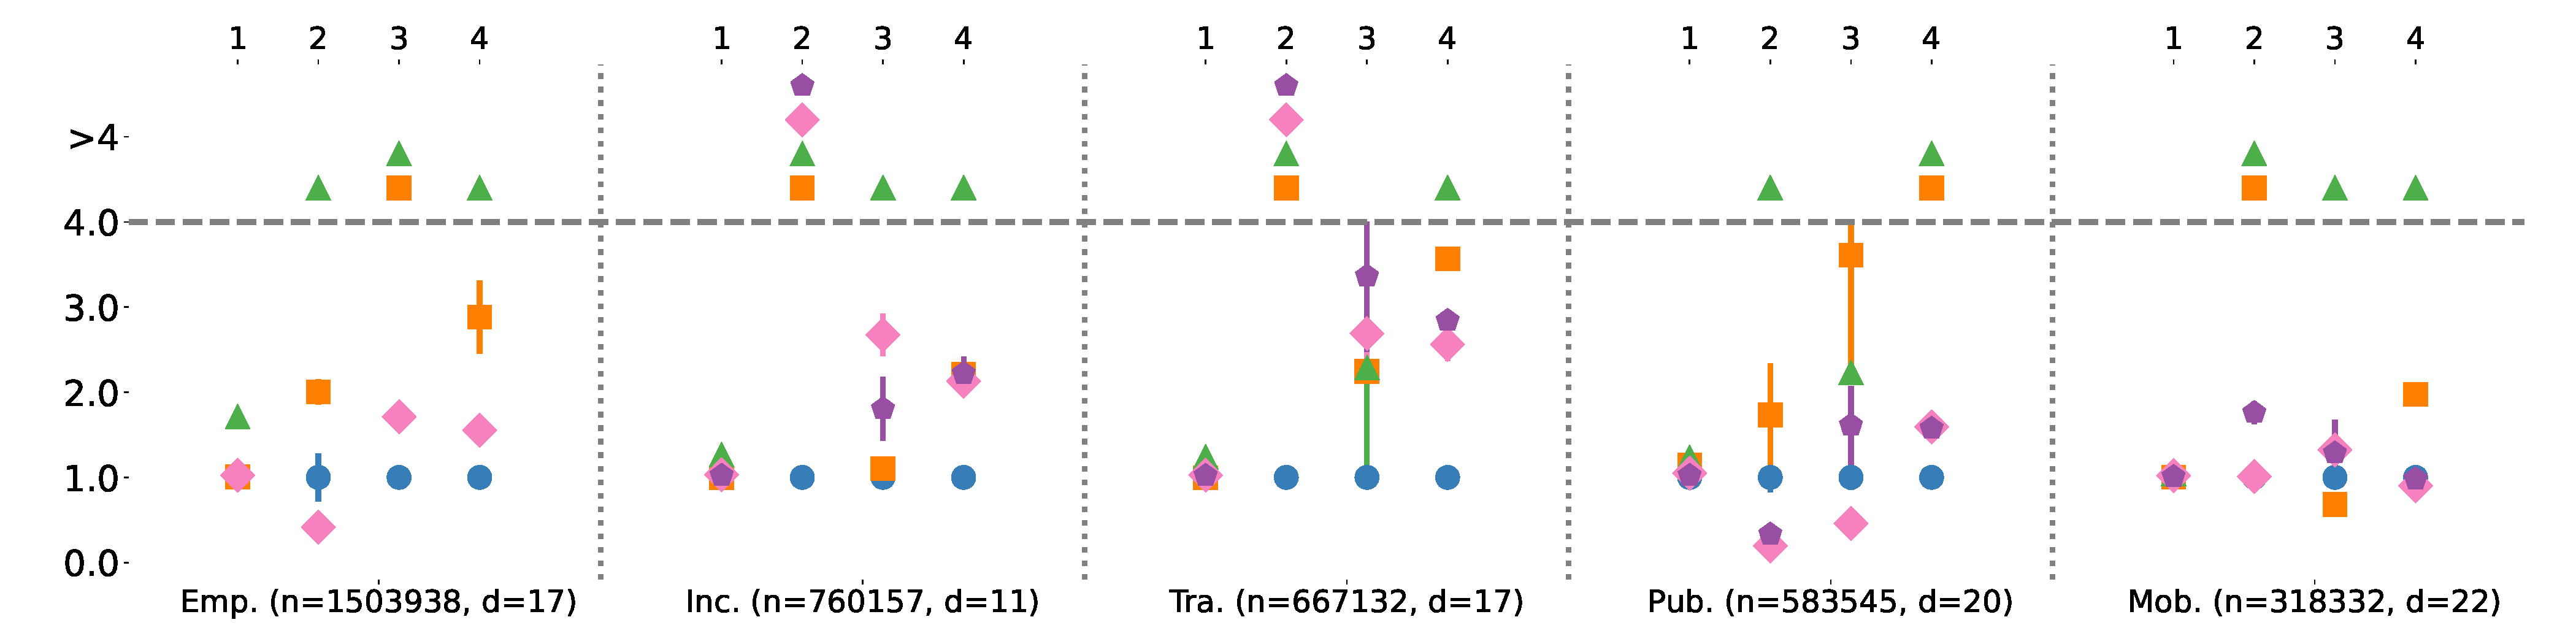
\includegraphics[width=\textwidth]{papers/PrivPGD/figures/plots_datasets/eps_2.5/1.pdf}\\[0.8ex]
  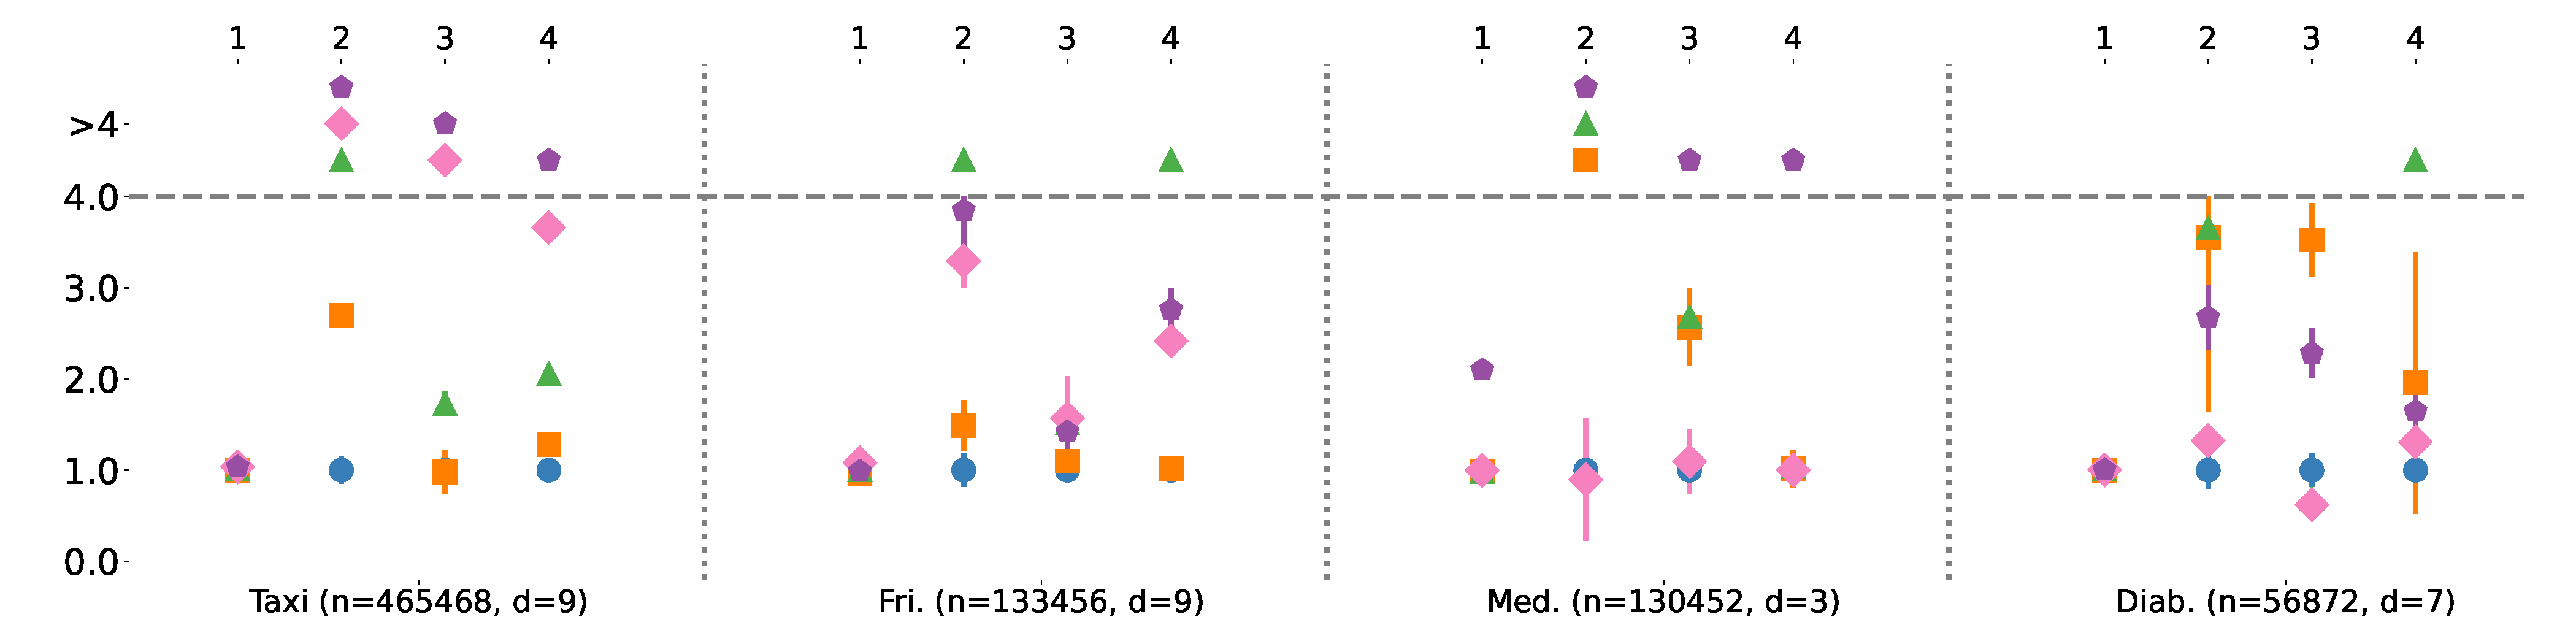
\includegraphics[width=\textwidth]{papers/PrivPGD/figures/plots_datasets/eps_2.5/2.pdf}
  \caption{Comparison of PrivPGD with state-of-the-art methods using all two-way marginals across nine tabular datasets. For each method, the figure reports the \(\log_2\) ratio of the errors relative to PrivPGD on downstream error, covariance error, counting query error, and threshold query error, averaged over five runs at \(\epsilon = 2.5\) and \(\delta = 10^{-5}\).}
  \label{fig:comp}
\end{figure}

\paragraph{Baselines.}
We benchmark PrivPGD against representative marginal-based and query-based methods. The marginal-based baselines are MST and AIM \citep{mst,aim}. The query-based baselines are Private GSD, RAP, and GEM \citep{pmlr-v202-liu23ag,aydore2021differentially,liu2021iterative}. Complete implementation details for PrivPGD and the baselines are deferred to Appendix~\ref{app:privpgd-implementation}.

\subsection{Main Benchmark Findings}

We now present how the performance of PrivPGD compares against state-of-the-art algorithms for differentially private data synthesis. The main comparison figure illustrates the relative performance of PrivPGD compared to other methods across the benchmark datasets and metrics. Overall, PrivPGD consistently ranks as either the best or the second-best method in most metrics and datasets, with a few exceptions such as the covariance error on the ACS Public Coverage dataset.

\paragraph{Comparison with PGM.}
PrivPGD systematically outperforms both variants of PGM, which are the state-of-the-art for marginal-based tabular data synthesis, often by a significant margin. In particular, it is better than PGM+MST in covariance and query errors across datasets, except for threshold query error on the Diabetes dataset, and performs at least as well as PGM+AIM in most settings, with the notable exception of threshold query error on the ACS Mobility dataset. For downstream tasks, PrivPGD performs comparably to PGM+AIM and consistently better than PGM+MST.

\paragraph{Comparison with query-based algorithms.}
PrivPGD is also the preferred method in most scenarios when compared to query-based approaches, especially against GEM and RAP. While Private GSD provides competitive performance and occasionally surpasses PrivPGD on specific datasets, such as ACS Public Coverage, PrivPGD usually emerges as the best-performing method. On many datasets, including Taxi, Black Friday, and ACS Traveltime, it significantly outperforms Private GSD across the reported metrics.

\FloatBarrier

\subsection{Geometry-Aware Fidelity}

\begin{figure}[!t]
  \centering
  \begin{minipage}{0.495\textwidth}
    \centering
    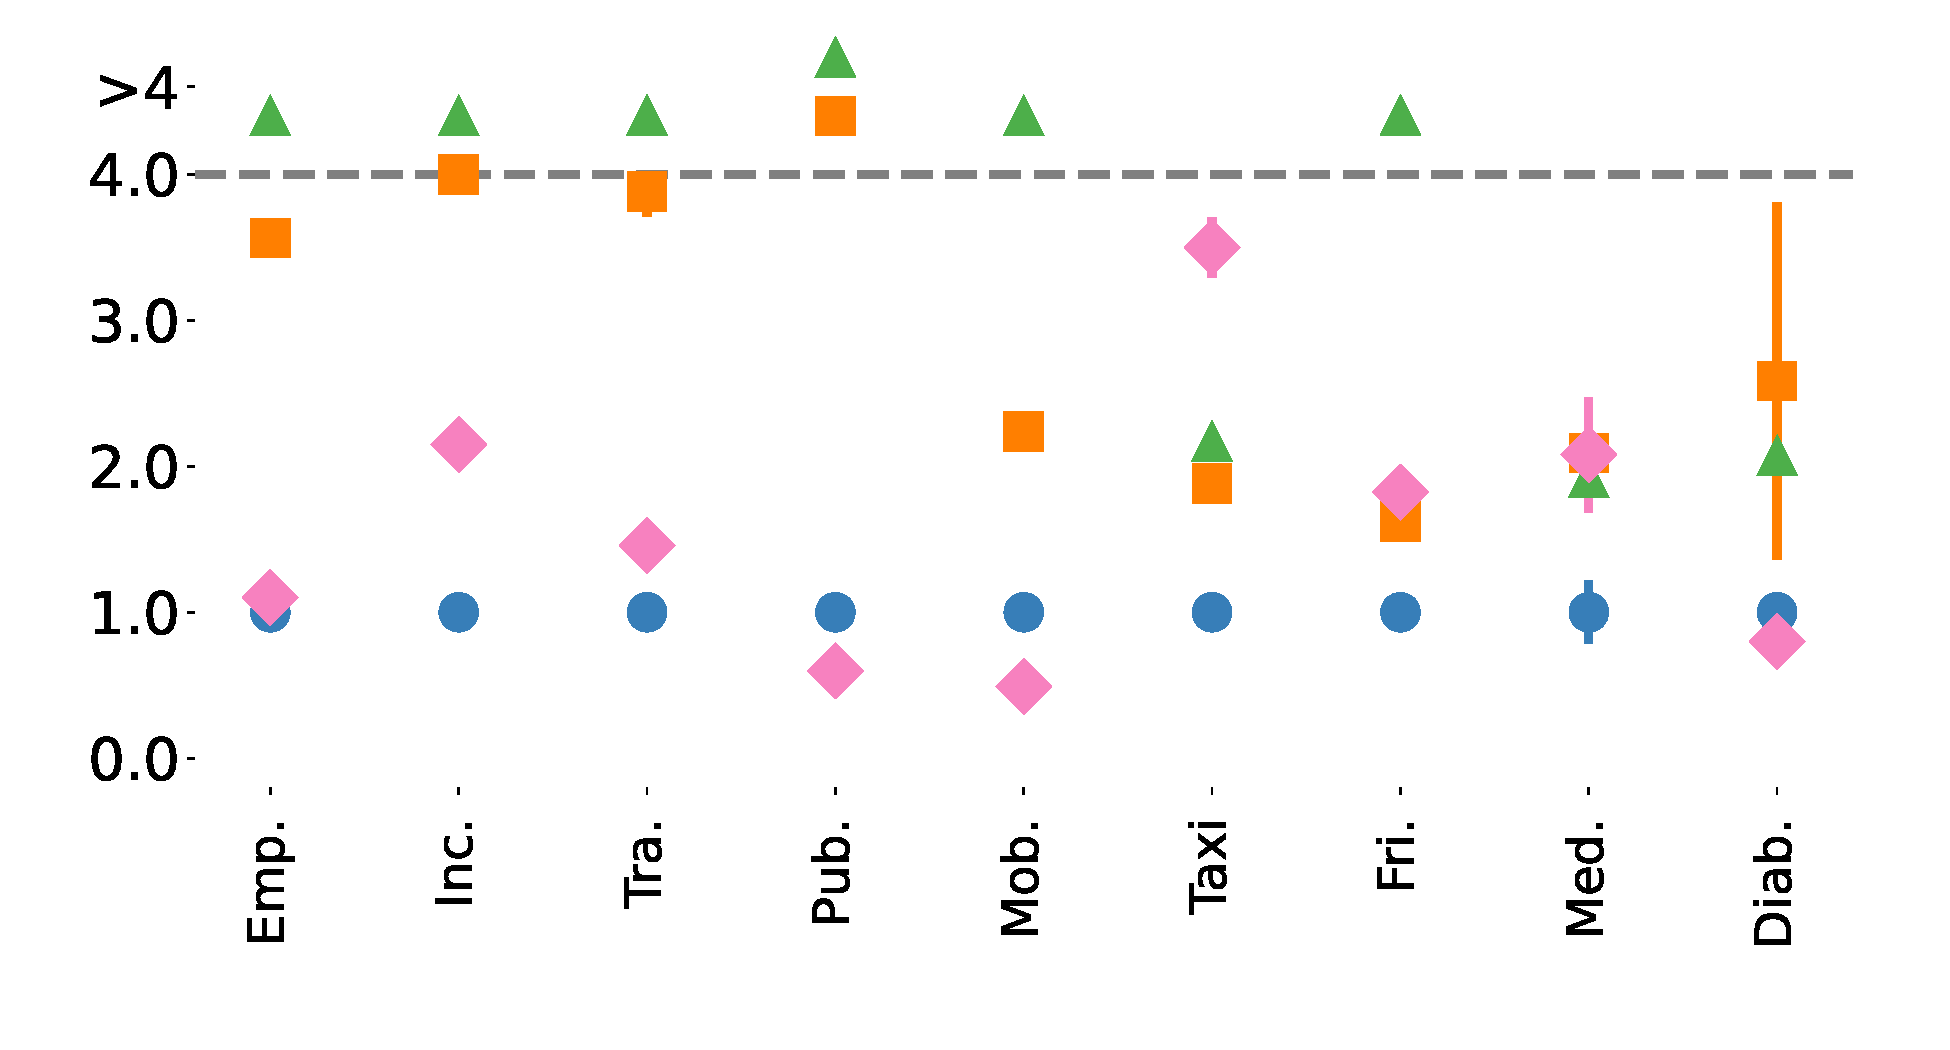
\includegraphics[width=\textwidth]{papers/PrivPGD/figures/plots_distances/eps_2.5/wdist_1_2Way_avg.pdf}
  \end{minipage}
  \hfill
  \begin{minipage}{0.495\textwidth}
    \centering
    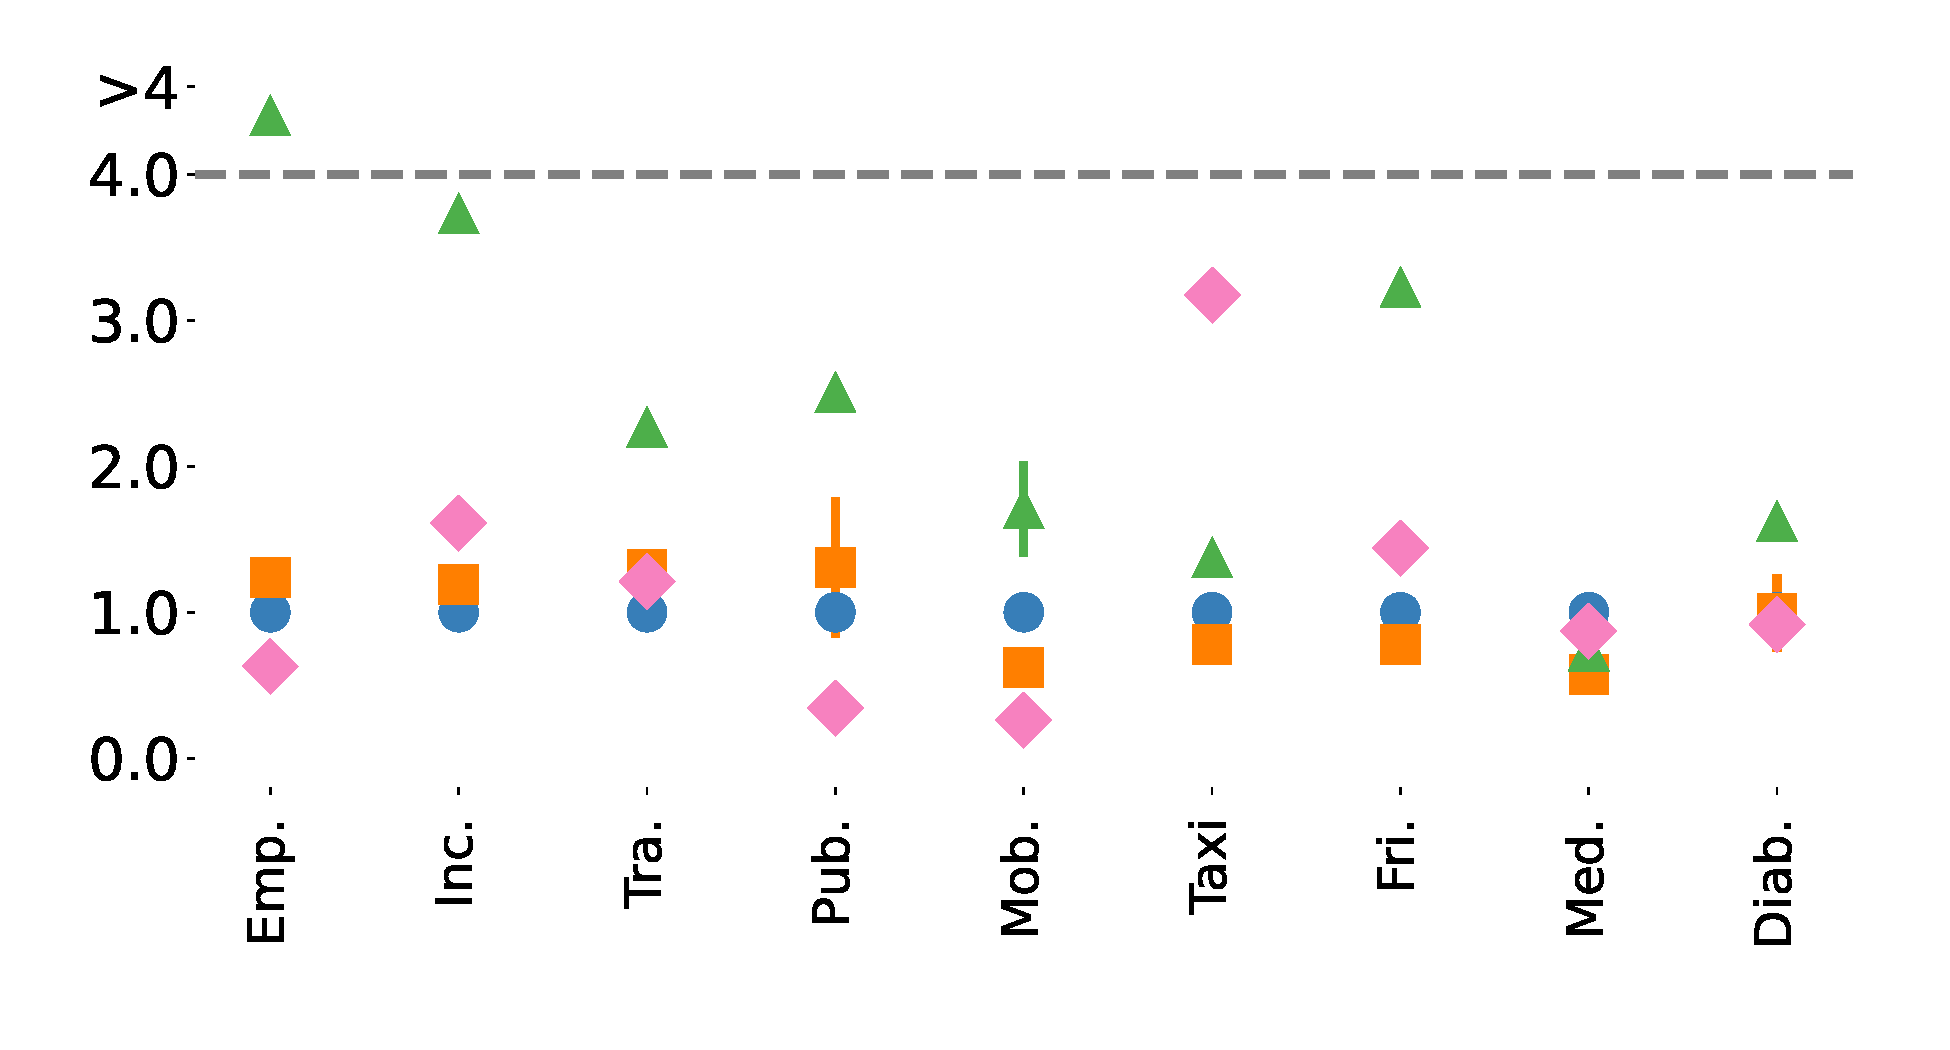
\includegraphics[width=\textwidth]{papers/PrivPGD/figures/plots_distances/eps_2.5/newl1_2Way_avg.pdf}
  \end{minipage}
  \caption{Comparison of average sliced Wasserstein distance (left) and average total variation distance (right) for PrivPGD against state-of-the-art methods across the benchmark datasets. As expected, PrivPGD compares especially well under the geometry-aware sliced Wasserstein metric that it directly optimizes.}
  \label{fig:comp-sw-tv}
\end{figure}

The comparison between sliced Wasserstein distance and total variation distance is particularly informative. It illustrates a noticeable performance gap between PrivPGD and other methods when comparing the average sliced Wasserstein distance and the total variation distance. PrivPGD effectively minimizes the former, while state-of-the-art methods like PGM primarily target the latter. This is the expected behavior: PrivPGD is optimized for a geometry-aware loss, and it therefore compares especially well under a geometry-aware notion of fidelity.
\FloatBarrier

\subsection{Domain-Specific Constraints}

\begin{figure}[!t]
  \centering
  \begin{minipage}{0.76\textwidth}
    \centering
    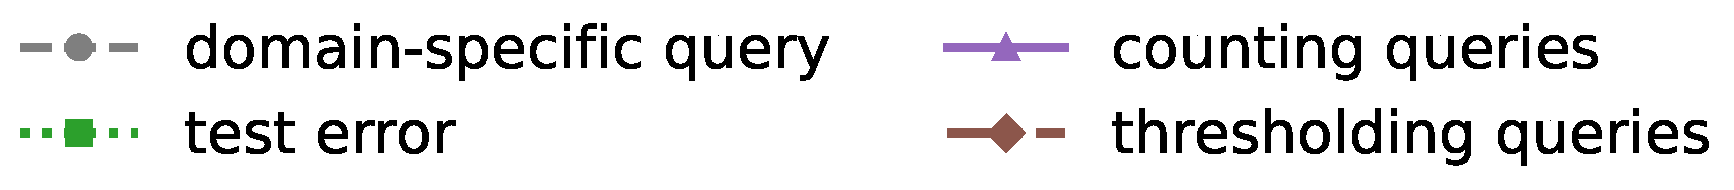
\includegraphics[width=0.82\linewidth]{papers/PrivPGD/figures/plots_constraint/exp3_legend.pdf}\\[0.6ex]
    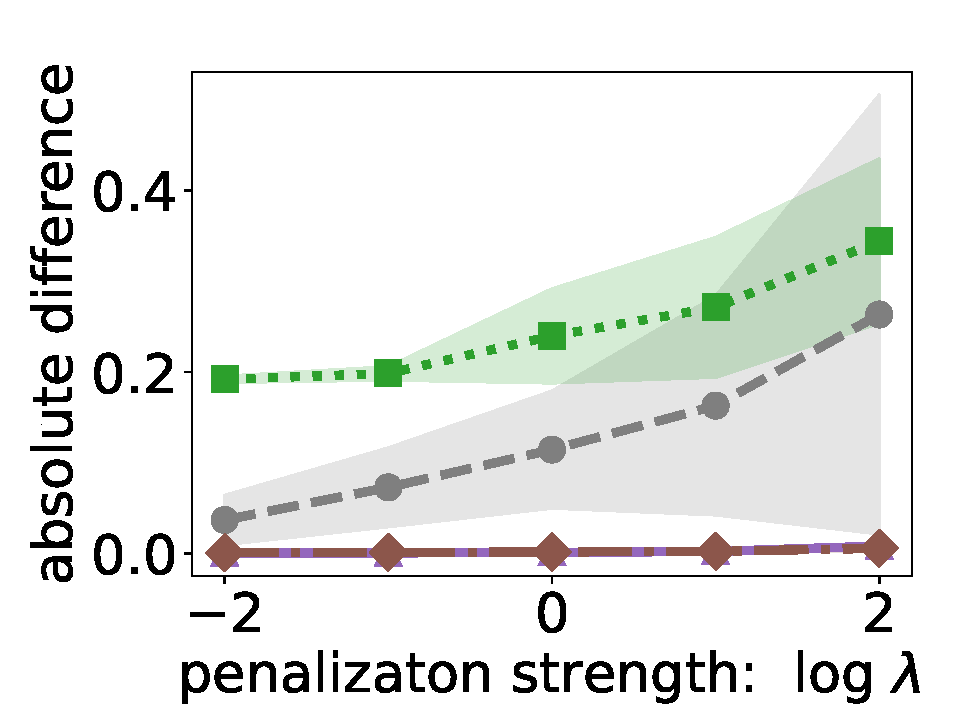
\includegraphics[width=0.48\linewidth]{papers/PrivPGD/figures/plots_constraint/exp3_acs_income_CA_2018_default_32+thresholding_1.pdf}
    \hfill
    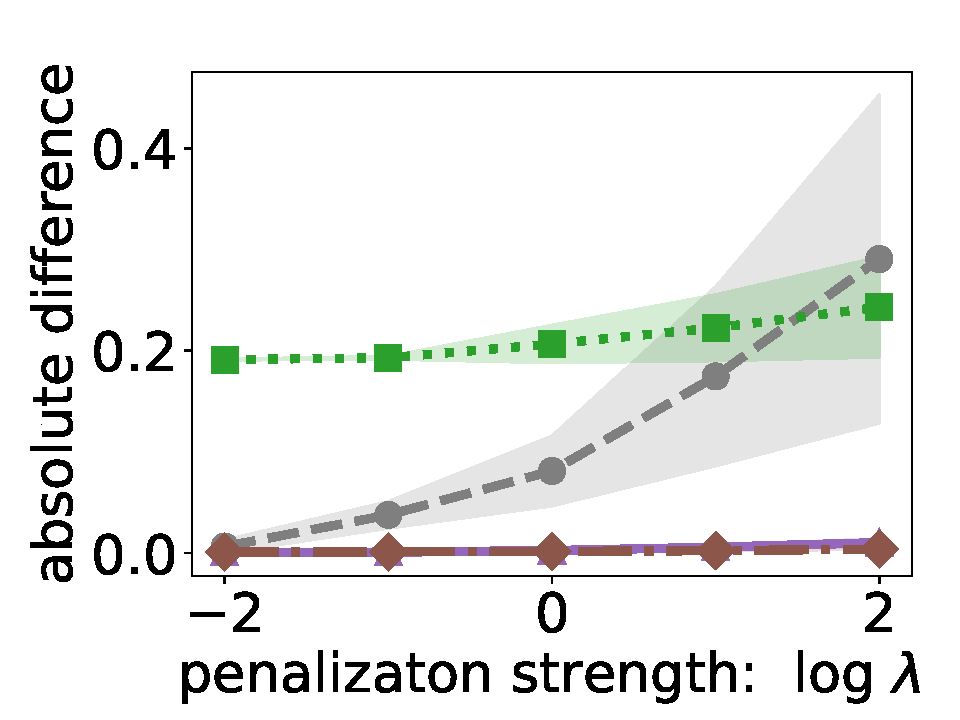
\includegraphics[width=0.48\linewidth]{papers/PrivPGD/figures/plots_constraint/exp3_acs_employment_CA_2018_default_32+thresholding_1.pdf}
    \caption{Effect of the domain-specific regularizer on the targeted threshold statistic, downstream performance, and unrelated random query errors for the ACS Income and ACS Employment datasets as a function of the regularization strength \(\lambda\).}
    \label{fig:constraints-main}
  \end{minipage}
\end{figure}

The final experiment shows that PrivPGD can protect population-level statistics while still constructing a high-quality dataset. While differential privacy protects individual information, many applications also require the protection of specific population-level statistics. In such cases, one would like selected statistics of the synthetic dataset to differ substantially from the corresponding statistics of the original data. One example is census data, where it might be desirable to hide religious or sexual orientations at the subpopulation level to prevent potential discriminatory misuse. Another example is the publication of rental and house sale prices, where exposing certain correlations could lead to speculative abuses in specific locales.

As an example, we consider maximizing the distance of a single linear non-sparse thresholding query defined directly in the embedding space. This query is approximated by a differentiable sigmoid surrogate, and the resulting differentially private regularization term is added to the objective. The exact construction is given in Appendix~\ref{app:privpgd-constraints}.

The resulting curves show that the targeted query is well approximated when no, or only little, regularization is used, and that increasing the regularization strength increasingly protects these statistics, as the domain-specific query on the synthetic dataset deviates strongly from the same query on the original data. At the same time, the downstream error and the errors on unrelated random counting and threshold queries remain comparable to the unregularized case even for relatively large regularization strengths. This illustrates that PrivPGD can incorporate domain-specific constraints in a direct and effective way.

\FloatBarrier

\section{Chapter Summary}

We introduced PrivPGD, a novel generation method for marginal-based private data synthesis. The approach leverages particle gradient descent together with tools from optimal transport, resulting in improved performance in a large number of settings, enhanced scalability for handling many marginals and larger datasets, and increased flexibility for accommodating domain-specific constraints compared to existing methods.

% The main chapter has focused on the core method and on the strongest empirical evidence. Extended dataset descriptions, lower-\(\epsilon\) results, full implementation details, and detailed benchmark tables are collected in Appendix~\ref{app:privpgd-datasets} through Appendix~\ref{app:privpgd-tables}, so that the main text can remain centered on the primary methodological and empirical contributions.
